\documentclass[UTF8, a4paper]{ctexart}
\usepackage{color}
\usepackage{anyfontsize}
\usepackage{extarrows}
\usepackage{amsthm}
\usepackage{caption}
\usepackage{geometry}
\usepackage{listings}
\usepackage{graphicx}
\usepackage{subfigure}
\usepackage{mathabx}  
\usepackage[ruled,linesnumbered]{algorithm2e}
\usepackage{amsmath} 
\usepackage{amsfonts,amssymb}

\geometry{left = 2.18cm, right = 2.18cm, top = 1.54cm, bottom = 1.54cm}

\begin{document}
\definecolor{grey}{RGB}{125, 125, 125}
\definecolor{MyGreen}{RGB}{0, 125, 0}
\centerline{\textbf{\LARGE{操作系统实验报告Lab2}}}
\bigskip
\centerline{\large{成员:陈豪斌 \quad 朱浩泽 \quad 许佳培}}

\begin{enumerate}
    \item [一、] \textbf{实现First Fit算法}
    \par
    首先我们需要分析代码中是如何组织空闲内存块的。
    实际上在代码中并非单独创建某个结构体用以表示block,而是定义了一个叫做Page的结构,然后以每个block的基址Page来标识各个块,作为它们的Identifier。
    这样的话就可以支持地址的比较了,因为,我们只需要定义一个指向Page的指针即可。指针的值就是它指向的元素的地址,因此,地址的比较可以在指针的运算的基础上完成。详情可见下图:
    \begin{figure}[!htb]
        \centering
        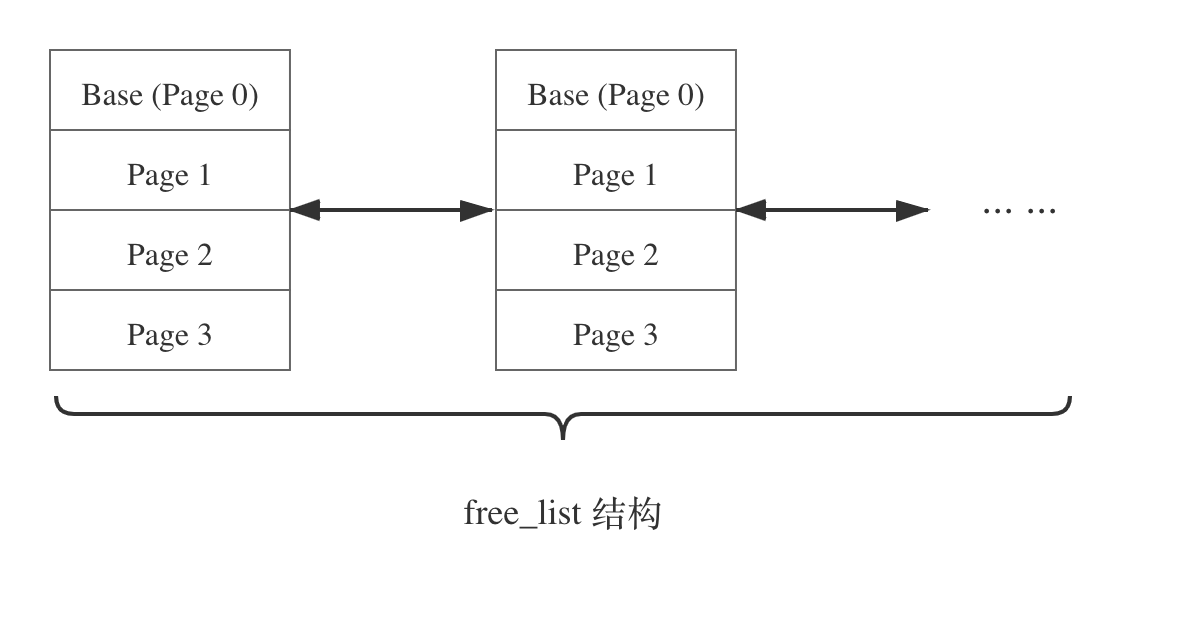
\includegraphics[scale=0.25]{freelist.png}
        \label{fig:1}
        \caption{free\_list和空闲内存块}
    \end{figure}
    \par
    例如,假设我们想要访问block 1中的page 2,我们先要设置一个指针指向free\_list的开始位置,随后将每个list\_entry类型的指针,通过一个叫做
    le2page的函数转换为page后判断property,然后设置基址指针为它,在基址的基础上增加偏移量即可访问任意page。随后的free和alloc函数也是基于指针和指针
    与page之间的转换而实现的。如果想要将page作为遍历free\_list的指针使用,就可以直接利用它的成员变量list\_link即可。
    \par
    对各个函数的模块功能解释:
    \begin{enumerate}
        \item [1.] 有关defualt\_init函数:它初始化free\_list。这个过程很简单,它把头尾指针都指向自身即可;
        \item [2.] 有关defualt\_init\_memmap函数:在一个块被分配之后我们需要把它进行初始化。因此它遍历块中的各个page,将其状态都设置为空闲,把reference标志位清空等。
                   特别地,如果page恰好是这个块的初始页,那么我们需要将其的property设置成块的大小。 因为我们想要实现FF算法,所以,必须要根据地址进行排序,那么通过指针比较即可实现这个
                   地址排序功能。此处就须将每个初始化好的块放置到free\_list的起始部分。
        \item [3.] 有关default\_alloc\_mem
    \end{enumerate}
\end{enumerate}

\end{document}